\documentclass[twocolumn, 8pt]{article}
\usepackage[greek,francais]{babel}
\newcommand\tet{\textgreek{tetraf'armakos}~}
\newcommand\IdC{I\textsuperscript{2}C~}
\newcommand\Ard{\textbf{\emph{Arduino}}~}
\newcommand\XB{\emph{XBee}~}
\newcommand\Xctu{\textbf{\emph{X-CTU}}~}
\newcommand\Att{\textbf{\emph{Attention:}}~}
\usepackage{eurosym}
\usepackage[T1]{fontenc}
\usepackage[utf8]{inputenc}
\usepackage[top=2cm, bottom=2cm, left=1cm, right=1cm]{geometry}
\setlength{\columnsep}{1cm}
\usepackage[usenames,dvipsnames]{color}
\usepackage{listings}
\lstset{language=C,
basicstyle=\ttfamily\small,
keywordstyle=\color{Blue}\bfseries,
identifierstyle=,
commentstyle=\color{Gray},
stringstyle=\color{BrickRed}\ttfamily,
morecomment=[l][\color{Green}]{\#},
showstringspaces=false,
tabsize=2,
numbers=left
}
\usepackage{graphicx}
\usepackage{amsmath,amssymb,amsfonts}
\usepackage{hyperref}

\title{Tutoriel de fabrication du \tet}
\author{Clément Javerzac-Galy \and{Denis Savoie}\\
	\texttt{\url{http://cansat2012.supop.fr}}
\and{Zubair Iftikhar}
}
\date{\today}

\begin{document}

\maketitle

\begin{abstract}
    \begin{bfseries}
	    \par \small Le projet \tet \footnote{pronouncez \textit{tetrapharmakos}} est un projet de Cansat réalisé par l'équipe des \textit{Proton-thérapeutes} de l'Institut d'Optique \textit{Graduate School} afin de participer au \textit{C'Space}, une compétition internationale co-organisée par Planète-Sciences et le CNES. 
	    \par \small Ce prototype de sonde spatiale embarque un module de mesure de l'indice de végétation fait-maison. Il enregistre en outre certains paramètres de vol à l'aide de divers capteurs (météorologiques et positionels).
    \par \small Nous espérons que toutes ces données mesurées permettront de caractériser les chances de présence de vie sur une exo-planète semblable à la Terre.
    \par \small Dans ce tutoriel, vous apprendrez à utiliser les différents composants que nous avons embarqués dans notre Cansat. Vous verrez comment tester le matériel, enregistrer les données mesurées sur une carte $\mu$SD et transférer des données à votre PC \textit{via} une liaison sans-fil.
     \end{bfseries}
\end{abstract}

\section{Matériel nécessaire}
Si vous souhaitez réaliser une copie exacte de notre projet (dont le coût total est d'environ 368\euro), il vous faudra:
\begin{enumerate}
	\item Contrôle et calculs:
		\begin{itemize}
			\item 2 x Micro-controlleurs Arduino Mini, 2 x 17\euro
			\item 1 adaptateur Arduino-Mini -- USB, 15\euro
		\end{itemize}
	\item Alimentation \footnote{Pour commencer, vous pouvez utiliser l'alimentation de la liaison USB entre votre Arduino et votre ordinateur.}
		\begin{itemize}
			\item 1 batterie 9V (NiMH), 13\euro
			\item 1 circuit d'adaptation de tension délivrant du 3,3V et du 5V, 5\euro
		\end{itemize}
	\item Stockage d'information
		\begin{itemize}
			\item 2 modules pour carte $\mu$SD, 2 x 13\euro
			\item 2 cartes $\mu$SD, 2 x 7\euro
		\end{itemize}
	\item Transfert de données sans-fil
		\begin{itemize}
			\item 2 modules XBee Pro, 2 x 36\euro 
			\item 1 \textit{dongle}-USB XBee, 21\euro
		\end{itemize}
	\item Capteurs
		\begin{itemize}
			\item 1 capteur d'humidité et température [RHT03], 15\euro
			\item 1 capteur de pression et température [BMP085], 18\euro
			\item 1 accéléromètre [ADXL345], 22\euro
			\item 1 module GPS [EM-406A], 29\euro 
			\item 2 caméras Jpeg [LinkSprite Jpeg TTL], 2 x 42\euro
		\end{itemize}
\end{enumerate}

\par Nous utilisons des composants en double car nous avons besoin de prendre deux photographies simultanées pour réaliser notre mesure de l'indice de végétation. Vous préfèrerez sans doute une Arduino Nano à une Mini, puisqu'elle est plus simple à programmer et à connecter à un ordinateur. Si vous voulez réduire les coûts et les contraintes techniques, voici la liste de composants à utiliser:
\begin{enumerate}
	\item Contrôle et calculs:
		\begin{itemize}
			\item 1 Micro-controlleurs Arduino Nano, 29\euro
		\end{itemize}
	\item Alimentation
		\begin{itemize}
			\item 1 batterie 9V (NiMH), 13\euro
			\item 1 circuit d'adaptation de tension délivrant du 3,3V et du 5V, 5\euro
		\end{itemize}
	\item Stockage d'information
		\begin{itemize}
			\item 1 modules pour carte $\mu$SD, 13\euro
			\item 1 cartes $\mu$SD, 7\euro
		\end{itemize}
	\item Transfert de données sans-fil
		\begin{itemize}
			\item 2 modules XBee, 2 x 26\euro 
			\item 1 \textit{dongle}-USB XBee, 21\euro
		\end{itemize}
	\item Capteurs
		\begin{itemize}
			\item 1 capteur d'humidité et température [RHT03], 15\euro
			\item 1 capteur de pression et température [BMP085], 18\euro
			\item 1 accéléromètre [ADXL345], 22\euro
			\item 1 module GPS [EM-406A], 29\euro 
			\item 1 caméras Jpeg [LinkSprite Jpeg TTL], 42\euro
		\end{itemize}
\end{enumerate}
Ce qui revient alors à 266\euro environ. Vous pouvez très bien adapter ce tutoriel à vos envies et choisir de faire une simple station météo (100\euro), ou un système de prise de photographies géolocalisées (138\euro).

\section{Assemblage et vérification du matériel}

\par Nous allons commencer par vérifier l'état de marche de chacun des composants. N'utilisez pas de pile au départ, l'alimentation se fera grâce à l'ordinateur. Par exemple si vous avez une Arduino Nano, il suffit de la connecter à votre ordinateur \textit{via} un câble USB (si vous utilisez une Arduino Mini, vous devez utiliser l'adaptateur Arduino FTDI USB-Série pour alimenter et programmer votre système).


\subsection{Le micro-contrôleur}
\par Pour savoir comment connecter votre Arduino à votre ordinateur pour la programmer, vous pouvez vous rendre sur le site officiel du fabricant: 
\begin{itemize}
	\item Arduino Mini: \url{http://arduino.cc/en/Guide/ArduinoMini}
	\item Arduino Nano: \url{http://arduino.cc/en/Guide/ArduinoNano}
\end{itemize}

\par \Att Veillez à NE PAS brancher votre Arduino en inversant les polarisations + et --.
\par Dans tous les cas, vous devez télécharger le logiciel de programmation \Ard sur \url{http://arduino.cc/en/Main/Software}. Utilisez le programme d'exemple \textsf{'Blink'} pour vérifier l'état de marche de votre micro-contrôleur.


\subsection{Le stockage sur carte $\mu$SD}
\par La plupart des applications nécessitent un enregistrement sur carte SD. Le prix de ces cartes mémoire Flash a beaucoup diminué, et on peut aujourd'hui facilement trouver une carte $\mu$SD de 2Go pour moins d'une dizaine d'euros. Il est recommandé d'utiliser des cartes de marque (j'avais une carte générique qui n'était pas reconnue, bien qu'elle soit bien formattée).

\par La figure \ref{SD} montre comment connecter le module de carte $\mu$SD à une Arduino Mini \footnote{Il faut savoir que les cartes SD doivent être alimentées en 3,3V, et que l'Arduino Mini fonctionne en 5V.}.

\begin{figure}[!h]
	\centering
	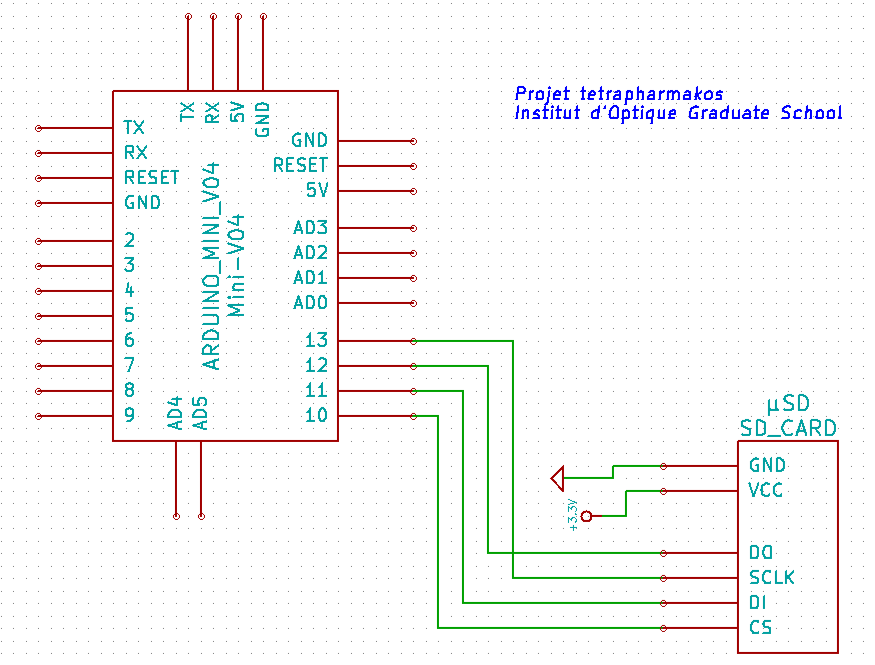
\includegraphics[scale=.25]{SD.png}
	\caption{Branchement d'une carte SD à une Arduino}
	\label{SD}
\end{figure}

\par Il faut alors utliser le programme d'exemple \textsf{'CardInfo'} du logiciel \Ard pour vérifier l'état de votre carte SD et de votre branchement.


\subsection{Les capteurs}
\par Notre Cansat devait remplir deux missions (sondage atmosphérique et mesure de l'indice de chlorophille). Pour la première, nous avions besoin d'un capteur d'humidité et d'un capteur de pression. Pour la seconde, nous avions besoin de deux caméra. L'accéléromètre et le module GPS étaient utilisés en vue de préparer une troisième mission: le atterissage maîtrisé sur une cible.

\subsubsection{Capteur d'humidité}
\par Le capteur d'humidité que nous avons utilisé est le \emph{RHT03}. Comme le reste des capteurs que nous avons utilisés, il est très simple d'emploi. La figure \ref{RHT03} montre comment le brancher \footnote{Il faut utiliser une résistance de tirage de 10k$\Omega$ entre la broche \no{}2 et l'alimentation +5V.}.

\begin{figure}[!h]
	\centering
	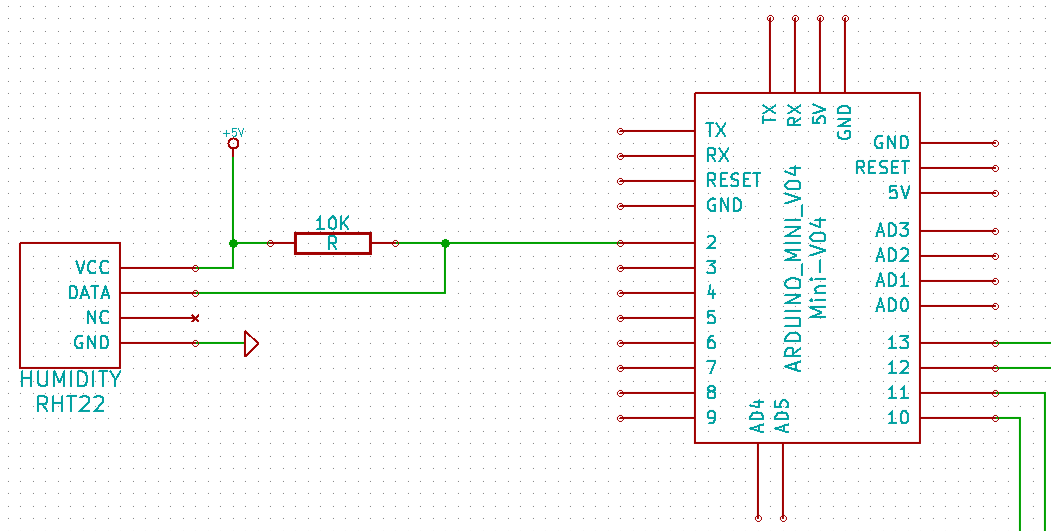
\includegraphics[scale=.2]{RHT03.png}
	\caption{Branchement du RHT03 à une Arduino}
	\label{RHT03}
\end{figure}

\par Il faut ensuite programmer votre micro-contrôleur pour envoyer les données du capteur sur le port Série de votre Arduino. Pour cela, téléchargez le programme \textsf{'DHTtester'} à l'adresse suivante: \url{https://github.com/thriller91/Cansat-SupOp/tree/master/sources/Arduino/DHT22/DHTtester}. Il faut télécharger les trois fichiers (\texttt{DHTtester.pde}, \texttt{DHT.cpp} et \texttt{DHT.h}), et les placer dans un même dossier appellé \textbf{DHTtester}.

\subsubsection{Capteur de pression}
\par Notre capteur de pression est le \emph{BMP085}. Il se connecte en \IdC. Comme le montre la figure \ref{BMP085}, il faut donc utiliser les broches analogiques \no{}4 et 5 de l'Arduino.

\begin{figure}[!h]
	\centering
	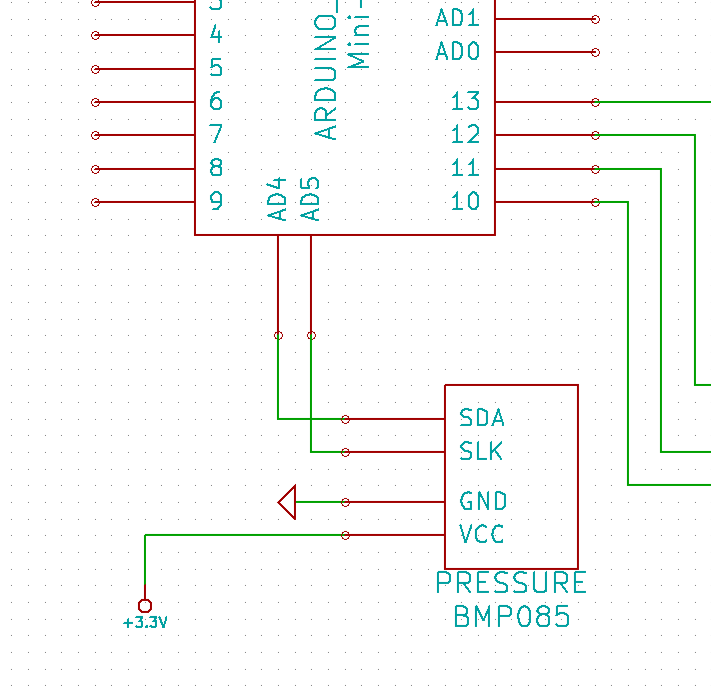
\includegraphics[scale=.2]{BMP085.png}
	\caption{Branchement du BMP085 à une Arduino}
	\label{BMP085}
\end{figure}

\par Le programme à télécharger pour essayer ce capteur est disponible à l'adresse suivante: \url{https://github.com/thriller91/Cansat-SupOp/tree/master/sources/Arduino/BMP085/BMP085tester}.

\subsubsection{Accéléromètre}
\par Nous avons utilisé un accéléromètre numérique, l'\emph{ADXL345}. Ce composant peut se connecter en \IdC ou en SPI (déjà utilisé par la carte SD). On peut connecter l'accéléromètre et le capteur de pression sur le même bus \IdC, mais comme nous avions 2 Arduino, nous avons utilisé une pour chaque capteur. Si vous voulez éviter d'utiliser une autre Arduino et que vous ne voulez pas placer ces deux composants sur le même bus, vous pouvez choisir d'utiliser un accéléromètre analogique (l'\emph{ADXL335} par exemple).

\par La figure \ref{ADXL345} montre comment brancher l'\emph{ADXL345} sur une Arduino en \IdC.

\begin{figure}[!h]
	\centering
	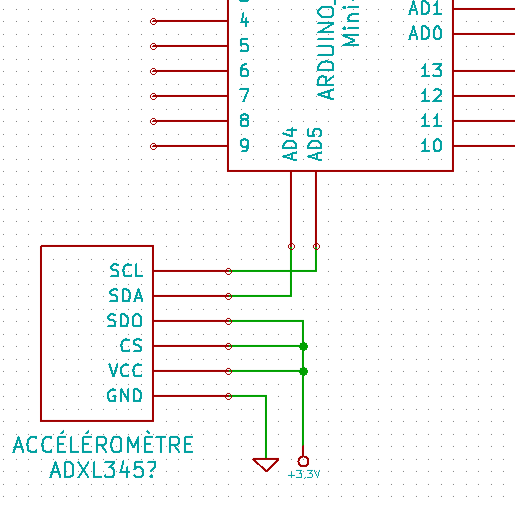
\includegraphics[scale=.25]{ADXL345.png}
	\caption{Branchement de l'ADXL345 en \IdC}
	\label{ADXL345}
\end{figure}

\par Le programme de pilotage de cet accéléromètre est disponible sur: \url{https://github.com/thriller91/Cansat-SupOp/tree/master/sources/Arduino/ADXL345/ADXL345tester}. Si vous utilisez l'accéléromètre analogique, il suffit de le connecter comme indiqué dans la documentation technique et d'utiliser le programme fournit dans les exemples du logiciel \Ard \textsf{'ADXL3xx'} (dans le dossier \textsf{Sensors}).

\par L'utilisation d'un accéléromètre seul (sans gyroscope) n'est pas idéale. Nous pensions pouvoir négliger les rotations du \tet pendant sa chute, mais nous avons rencontré un autre problème. Étant donné que la structure mécanique de notre Cansat n'était pas très rigide, elle a finie par s'incliner au fil du temps, et nous ne pouvions malheuresement plus compter sur notre capteur de pression pour déterminer l'angle de la verticale \footnote{En utilisant une formule du nivellement barométrique} (vous pouvez retrouver nos résultats dans notre présentation \url{http://cansat2012.supop.fr/presentation.pdf}). Si vous voulez enregistrer le véritablement mouvement de votre système, visitez la page suivante pour choisir votre centrale inertielle: \url{https://www.sparkfun.com/pages/accel_gyro_guide}.

\subsubsection{Module GPS}
\par Le module GPS \emph{EM-406A} n'est pas une simple antenne GPS. Ce composant est totalement autonome, il suffit de l'alimenter pour qu'il envoit ses trames GPS (NMEA) --- après s'être synchronisé avec les satellites bien évidemment. Il envoit ses données \textit{via} un port série à 4800 bauds. Il suffit donc de le brancher comme sur le schéma de la figure \ref{GPS}.

\begin{figure}[!h]
	\centering
	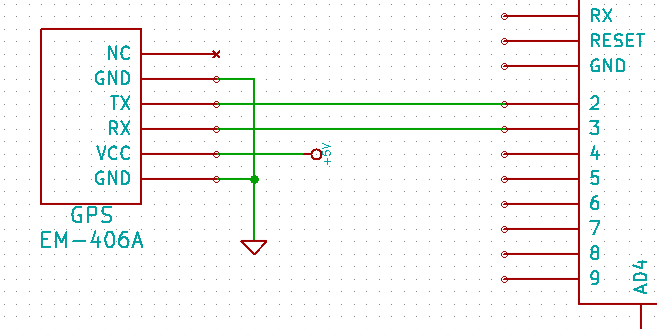
\includegraphics[scale=.25]{EM-406A.png}
	\caption{Branchement de l'EM-406A}
	\label{GPS}
\end{figure}

\par Des exemples de programmes d'utilisation sont disponibles dans la bibliothèque \textsf{TinyGPS}, que vous pouvez télécharger librement à l'adresse suivante: \url{http://arduiniana.org/TinyGPS/TinyGPS12.zip} \footnote{Dézippez ce fichier dans le dossier \textsf{libraries} d'\Ard, puisque ses exemples commencent par \lstinline$\#include <TinyGPS.h>$. Redémarrer ensuite \Ard pour pouvoir voir les programmes que vous venez de télécharger dans les exemples du logiciel.}
\par Ces programmes utilisent la bibliothèque \textsf{SoftwareSerial} d'\Ard. Elle permet de simuler un port série \{RX,TX\} sur des broches de la carte Arduino. Il suffit de créer un objet \lstinline$SoftwareSerial mySerial(2, 3); // RX, TX$ , pour que la broche \no{}2 (resp. \no{}3) de votre Arduino soit l'entrée (resp. la sortie) de votre port série.

\subsubsection{Caméra Série Jpeg}
\par Notre mission principale était la mesure de l'indice de chlorophylle, cette mesure passe par la capture deux photographies d'une même scène, chacune derrière un filtre optique. Notre problème était qu'il est difficile de trouver une caméra facile à interfacer avec notre micro-contrôleur. L'idéal est alors de choir une caméra avec une sortie série. Le prix de ce type de caméra peut sembler élevé --- environ le quadruple --- à côté d'une simple webcam, mais il est quasiment impossible de démonter le capteur d'une webcam pour s'en autrement qu'avec les pilotes logiciel fourni par le constructeur (et qui ne sont pas destinés aux micro-contrôleurs).
\par Nous avions commencé par utiliser une caméra Jpeg de 4DSystems, la \emph{$\mu$CAM-TTL}. Nous avions réussi à prendre des photographies en la pilotant sur ordinateur avec notre propre programme écrit en C. Mais la traduction de ce code en programme pour \Ard \footnote{Les programmes sont disponibles dans notre répertoire GitHub, dans la branche \textsf{$\mu$Cam-Z} sur \url{https://github.com/thriller91/Cansat-SupOp}.} ne permettait malheuresement pas de prendre des images avec le micro-contrôleur --- bien que nous arrivions à savoir que la caméra était bien synchrnoisée avec ce dernier.
\par Il fallait alors changer de caméra, nous avons donc choisit la caméra Jpeg de LinkSprite, la \emph{LinkSprite JPEG Color Camera TTL Interface}. Nous avons rapidement maîtrisé cette caméra, et nous l'avons connectée au port série natif de notre micro-contrôleur. Le branchement que nous avons fait est expliqué sur la figure \ref{camera}.

\begin{figure}[!h]
	\centering
	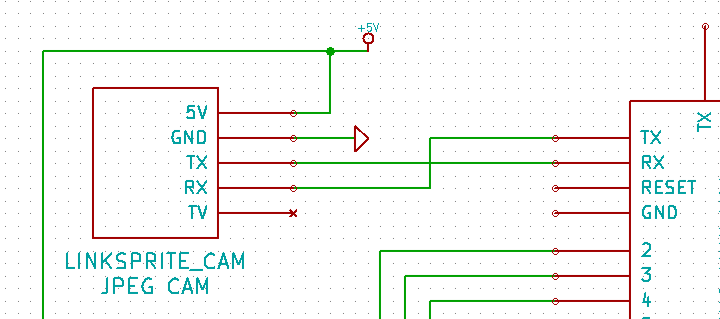
\includegraphics[scale=.25]{LinkSprite.png}
	\caption{Branchement de la caméra Jpeg LinkSprite}
	\label{camera}
\end{figure}

\par \Att Lorsque la caméra est branchée de cette façon, la carte Arduino ne peut pas être programmée, il faut débrancher la caméra pour pouvoir programmer votre micro-contrôleur.
\par Si vous êtes gêné par ce branchement, il vous est aussi possible de brancher la caméra sur deux autres broches de votre Arduino, et utiliser la bibliothèque \textsf{SoftwareSerial} d'\Ard.
\par Nous utilisons la carte SD pour stocker la photographie, puis nous attendons l'atterissage du \tet avant de transférer les informations à une station au sol. Le programme \textsf{spark} (que vous pouvez télécharger à l'adresse: \url{https://raw.github.com/thriller91/Cansat-SupOp/master/sources/Arduino/LinkSprite/exemples/spark/spark.ino} est très largement inspiré d'un exemple de code donné par un utilisateur de \href{http://www.sparkfun.com/}{SparkFun.com}, il prend une photographie et l'enregistre sur la carte mémoire. On peut relancer ce programme plusieurs fois, les images ne sont pas écrasées, elles sont renommée \textsf{IMGxx.JPG} sur la carte SD.
\par Avec ce programme, la capture d'une photo prend environ 5 secondes, et son enregistrement 20 secondes. Vous pouvez changer la résolution et taux de compression de l'image selon la qualité d'image que vous voulez, mais ces changements modifiront le temps d'exécution du programme. Il ne faut évidemment ni débrancher la carte mémoire, ni mettre la caméra ou le micro-contrôleur hors-tension avant la fin du programme; sinon, vous obtiendrez un fichier image de 0 octet de mémoire sur votre carte SD.
\par Pour récupérer l'image en utilisant ce programme, il faut glisser votre carte mémoire dans un adaptateur $\mu$SD-SD ou votre téléphone portable pour ouvrir directement le fichier image.


\subsection{Transfert de données sans-fil}
\par Une liaison sans-fil avec le Cansat était essentielle pour le projet \tet, nous simulons en effet l'\emph{atterissage} d'une sonde sur une planète extra-terrestre. Cette sonde doit pouvoir communiquer ses résultats à une station au sol. Nous utilisons pour ce faire un module appellé \XB. Ce module est basé un protocol similaire au Wifi. Il existe toute une gamme d'\XB, nous avons choisit d'utiliser des \emph{XBee-Pro S1} longue portée. L'une était branchée au micro-contrôleur, et l'autre à la station au sol \textit{via} un \emph{dongle} USB.
\par Pour commencer, il faut configurer les \XB pour qu'elles se connaissent entre elles. Il faut télécharger le logiciel \Xctu sur le site de \textbf{Digi}, il est uniquement disponible sous Windows. La documentation fournie permet de configurer rapidement son matériel. Notez bien la vitesse de la communication série (en baud).
\par Laissez une \XB branchée à votre ordinateur, et connectez l'autre à votre micro-contrôleur comme sur la figure \ref{XBee} \footnote{La distance entre deux broches de la \XB est de 2mm et non 2.54mm comme pour la plupart des composants électroniques, vous pouvez acheter un \emph{socket} pour éviter de souder directement sur la \XB.}.

\begin{figure}[!h]
	\centering
	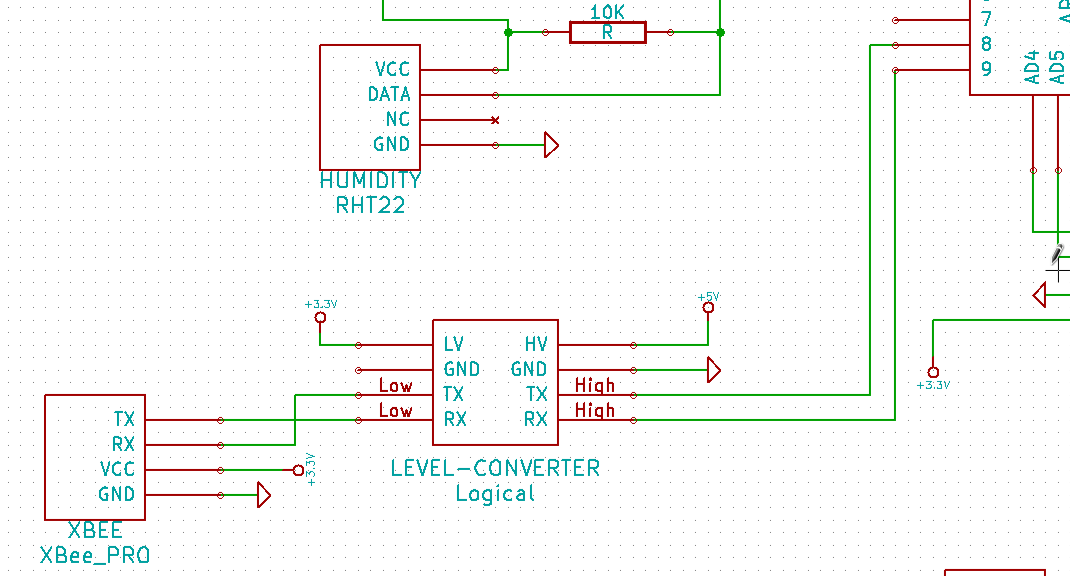
\includegraphics[scale=.25]{XBee.png}
	\caption{Branchement du module XBee}
	\label{XBee}
\end{figure}

\par \Att La chose à ne surtout pas faire avec votre \XB est de l'alimenter en inverse. Vous risquer de la tuer en quelques secondes --- croyez nous. Les \XB fonctionnent en 3.3V, et comme leur prix est assez élevé, il est sage d'utiliser un convertisseur de niveaux logiques pour l'interfacer avec une Arduino à 5V.

\par Il faut ensuite programmer votre micro-contrôleur pour qu'il envoit et reçoit des messages de la part de la station au sol. Vous pouvez commencer par charger un programme du dossier d'exemples \textsf{SoftwareSerial} du logiciel \Ard. Les deux \XB agissent comme des fils entre les RX et TX du convertisseur de niveau logique et le \emph{dongle} USB de la station au sol \footnote{Nous vous conseillons de commencer par utiliser des fils croisés entre les RX et TX de ces deux cartes, remplacez les fils par des \XB lorsque ça fonctionne.}
\par Vous savez maintenant communiquer sans-fil avec votre système. Vous pouvez donc recevoir les données qu'il vous envoit. Cependant, vous êtes dépendant du \textsf{moniteur série} d'\Ard. Vous aurez donc du mal à recevoir des données binaires --- comme des images par exemple. Pour vous affranchir du logiciel \Ard, vous pouvez choisir de rediriger le flot d'information vers un fichier, sous Linux, vous pouvez entrer \texttt{cat /dev/ttyUSB0 > reception.bin} dans un terminal \footnote{Saisir \textsf{Ctrl+C} pour arrêter la réception. Il faut remplacer \texttt{/dev/ttyUSB0} par le bon port. Vous pouvez aussi utiliser \texttt{screen} pour remplacer le \textsf{moniteur série} d'\Ard, il faudra alors entrer \texttt{screen /dev/ttyUSB0 9600} dans le terminal.}. Ce genre de solution est très simple, mais on ne voit le programme Arduino s'executer; en particulier, on ne sait pas quand il se termine. Si vous n'avez pas Linux, ou que vous vous voulez utiliser une méthode plus évoluée que la redirection de flot, vous pouvez télécharger notre programme Python à l'adresse suivante: \url{https://raw.github.com/thriller91/Cansat-SupOp/master/sources/prgm\%20sol/communication/pycrop/pycom.py}. Ce programme n'est qu'une ébauche, mais c'est celui que nous avons utilisé le jour de la comptétition, et nous avons réussi à récupérer notre image intacte \footnote{Pour l'anecdote, le \tet avait atterri dans un arbre et nous n'avions pu le récupérer qu'à la fin de la journée, mais cela ne nous a pas importuné.}.
\end{document}
